\section{Théorie}

Les cellules photovoltaïques sont composées de deux semi-conducteurs formant une jonction PN. Lorsque la lumière du soleil frappe la cellule photovoltaïque, elle génère des paires électron-trou dans la région de la jonction.
Les électrons dans la zone N sont poussés vers la jonction par le champ électrique créé par les charges fixes dans le matériau. Ces électrons se déplacent vers la zone P, créant ainsi un courant électrique \(I_\gamma\), comme illustré dans la figure \ref{fig:pn}.
Le courant \(I_D\) traversant la jonction PN est relié à la tension directe \(U_D\) [\unit{\volt}] par la relation \ref{eq:1} \cite{notice}:
\begin{equation}
    I_D = I_{SO}[e^{\alpha\frac{U_D}{T}} - 1] - I_\gamma
    \label{eq:1}
\end{equation}
où \(\alpha\) est une constante, \(T\) la température de la jonction en kelvins et \(I_{SO}\) le courant de saturation inverse de la jonction.

\begin{figure}
    \centering
    \begin{subfigure}[t]{0.45\linewidth}
        \centering
        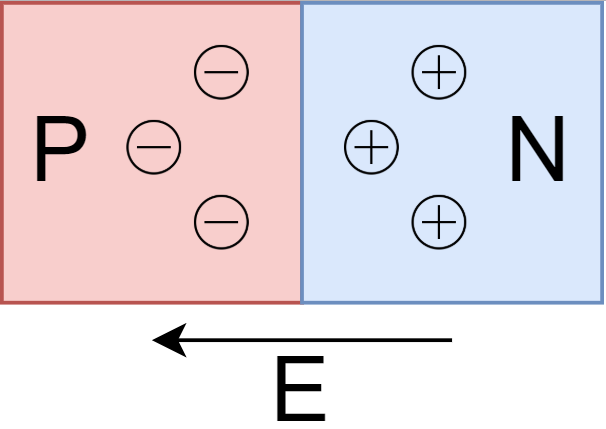
\includegraphics[width = 0.6\linewidth]{figures/junction1.png}
        \caption{Diagramme d'une jonction PN non illuminée. Le semi-conducteur P contient un excès de charge positives, des trous comme représenté ici, alors que N contient un excès de charges négatives, créant ainsi un champ électrique.}
    \end{subfigure}
    \hfill
    \begin{subfigure}[t]{0.45\linewidth}
        \centering
        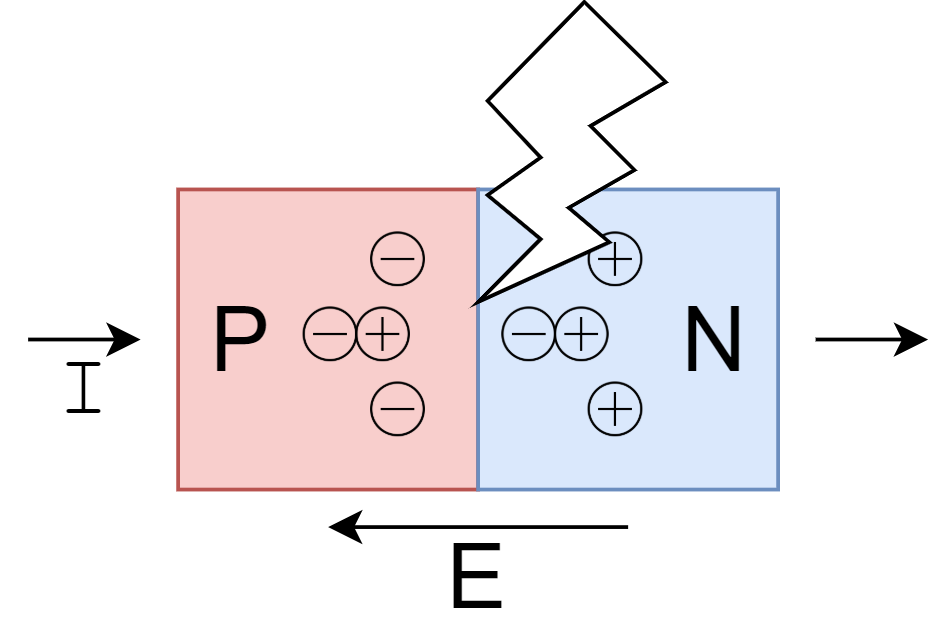
\includegraphics[width = 0.95\linewidth]{figures/junction2.png}
        \caption{Lorsque la jonction absorbe un photon, des charges électriques sont libérées. Sous l'effet du champ électrique régnant dans la jonction, les deux types de charges créées sont séparées et se répartissent, suivant leur
        polarité, de part et d'autre de la jonction, créant ainsi un courant \(I_\gamma\).}
    \end{subfigure}
    \caption{Illustration du fonctionnement d'une jonction PN \cite{nicole}}
    \label{fig:pn}
\end{figure}

Une jonction présente des comportements différents selon son eclairement: la photoconduction, le photovoltaïsme et la conduction directe.
Pour la génération d'énergie, le domaine interessant est celui du photovoltaïsme, où la jonction se comporte comme un générateur quand connecté à une résistance de charge \(R_C\).
Il existe une resistance de charge optimale \(R_{opt}\) pour laquelle la puissance de la cellule \(P = R_C I_R\) est maximale, et est notée \(P_{max}\), où \(I_R = -I_D\).

Le rendement énergétique \(\eta\) d'une cellule solaire est donnée par l'équation \ref{eq:2}:
\begin{equation}
    \eta = \frac{P}{P_\gamma}
    \label{eq:2}
\end{equation}
avec \(P\) la puissance de sortie de la cellule et \(P_\gamma\) la puissance solaire reçue sur la surface \(S\) de la cellule.
Le rendement maximal \(\eta_{max}\) est obtenu pour \(P = P_{max}\).
